\documentclass[12pt]{article}
\usepackage[margin=1in]{geometry}
\usepackage[x11names]{xcolor}
\usepackage{float}  
\usepackage{amsmath}
\usepackage{amssymb}
\usepackage{graphicx}
\usepackage{hyperref}
\usepackage{mdframed}
\usepackage{listings}

\lstset{
  basicstyle=\ttfamily,
  frame=single,
  numbers=left,
  numberstyle=\tiny,
  stepnumber=1,
  breaklines=true
}
\hypersetup{
    colorlinks=true,
    linkcolor=black,
    citecolor=blue,
    filecolor=blue,
    urlcolor=gray
}
\newmdenv[
  backgroundcolor=gray!10,
  linecolor=black,
  innerleftmargin=10pt,
  innerrightmargin=10pt,
  innertopmargin=10pt,
  innerbottommargin=10pt,
  roundcorner=5pt,
  linewidth=1pt,   
]{definitionbox}

\title{\textbf{Distributed Bitonic Sort with MPI}}
\author{Maria Charisi\\Maria Sotiria Kostomanolaki}
\date{\today}

\begin{document}

\maketitle

\begin{abstract}
    This project implements a distributed sorting program using \textbf{MPI}, based on the \texttt{Bitonic Sort} algorithm. The program sorts \( N = 2^{(q + p)} \) integers in ascending order across \( 2^p \) processes, each starting with \( 2^q \) random integers. It follows the \texttt{Bitonic Sort} method, combining local sorting and data exchange between processes to achieve the final result. The program validates the sorting and compares the performance of the parallel implementation for different values of \( q \) and \( p \). To evaluate the efficiency of the parallel approach, the program was tested on the Aristotelis cluster for high-scale performance as well as tested against \texttt{qSort} and serial \texttt{BitonicSort} to verify speedup achievement.
    
    You can find the source code of our implementation on this \href {https://github.com/mariaxarisi/Bitonic-Sort}{Github repository}.
\end{abstract}

\tableofcontents

\vfill
\begin{center}
    \textit{Professor: Nikolaos Pitsianis\\
    Department of Electrical and Computer Engineering\\
    Parallel and Distributed Systems}
\end{center}
\newpage

\section{Serial Bitonic Sort}

Understanding \texttt{Distributed Bitonic Sort}, requires a first examination of the concepts of a bitonic sequence, the Bitonic Theorem, and the serial implementation of the algorithm.

\subsection{Bitonic Sequence}

\begin{definitionbox}
A \textbf{Bitonic Sequence} is a sequence of integers that first increases monotonically and then decreases monotonically (or vice versa). The reverse of a bitonic sequence or any cyclic rotation of it also forms a bitonic sequence.
\end{definitionbox}

To elaborate on the last point with an example, the sequence [6, 4, 3, 1, 2, 5, 8, 7] is bitonic. When the last element, 7, is rotated to the beginning, the resulting sequence [7, 6, 3, 1, 2, 5, 8] satisfies the bitonic property.

\subsection{Bitonic Merge}

\begin{definitionbox}
\textbf{Bitonic Theorem:} The element-wise comparison of the first half of a bitonic sequence with its second half, along with the separation into minima and maxima subsequences, also results in bitonic sequences.
\end{definitionbox}

\textbf{Bitonic Merge} is an algorithm that takes a bitonic sequence with a length that is a power of two and returns a sorted sequence. \texttt{Bitonic Merge} recursively applies the \textit{Bitonic Theorem} and stores first the minima and then the maxima sequence, as demonstrated in the following example:

\begin{figure}[H]
    \centering
    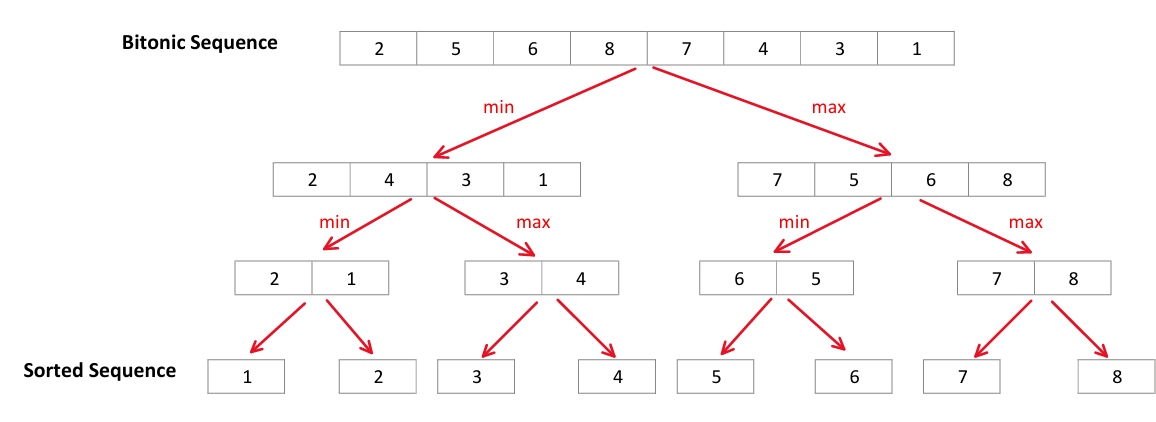
\includegraphics[width=0.9\linewidth]{serialBitonic.png}
    \caption{Bitonic Merge}
    \label{fig:enter-label}
\end{figure}

If we assume that the input sequence has length $n$, then:

\begin{itemize} 
\item Element-wise comparisons between the two halves of the sequence have a time complexity of $O(n)$.
\item \texttt{Bitonic Merge} calls itself twice: once for the minima sequence and once for the maxima sequence and it is recursively called $log(n)$ times. 
\end{itemize}

Below is the serial implementation of the \texttt{Bitonic Merge} algorithm, where \texttt{m} represents the size of the sequence or subsequence being processed in the current recursion and \texttt{min.arr[]} and \texttt{max.arr[]} are the respective minima and maxima subsequences.

\begin{lstlisting}[language=C]
    for(int i = 0; i < m; i++){
        if(arr[i] > arr[i+m]){
            min.arr[i] = arr[i+m];
            max.arr[i] = arr[i];
        } 
        else {
            min.arr[i] = arr[i];
            max.arr[i] = arr[i+m];
        }
    }

    min = bmerge(min, order);
    max = bmerge(max, order);
\end{lstlisting}
\vspace{0.3cm}
Therefore, the \textbf{time complexity} of \texttt{Bitonic Merge} is:
\[T_M(n) = 2T_M(n/2) + O(n) = O(nlog(n))\]

\subsection{Bitonic Sort}
\textbf{Bitonic Sort} takes an arbitrary sequence of integers as input and transforms it into a bitonic sequence. It achieves this by recursively dividing the sequence, sorting each half in opposite orders. Following that, it calls \texttt{Bitonic Merge} to merge the bitonic sequence into the desired order, resulting in a fully sorted sequence.
\vspace{0.3cm}
\begin{lstlisting}[language=C]
    l = bsort(l, true); //First half ascending order
    r = bsort(r, false); //Second half descending order

    // Create the bitonic sequence
    for(int i = 0; i < m; i++){
        b.arr[i] = l.arr[i];
        b.arr[i + m] = r.arr[i];
    }

    b = bmerge(b, order);
\end{lstlisting}
\vspace{0.3cm}
Taking into account the algorithm above, the \textbf{time complexity} of the \texttt{Bitonic Sort} is:

\[T_S(n) = 2 T_S(n/2) + T_M(n) = O(n (\log n)^2)\]

\newpage

\section{Distributed Bitonic Sort}

Although \texttt{Bitonic Sort} is a serial sorting algorithm and is slower than other similar algorithms, such as \texttt{Merge Sort} which has a time complexity of \(O(n \log n)\) compared to \texttt{Bitonic Sort}'s \(O(n (\log n)^2)\), it possesses useful properties that are well-suited for parallel and distributed implementations.

The \texttt{Distributed Bitonic Sort} takes two integers, \textbf{\( p \)} and \textbf{\( q \)}, as input. The algorithm sorts a sequence of \textbf{\( N = 2^{(q + p)} \)} integers in ascending order across \textbf{\( 2^p \)} processes, with each process starting with \textbf{\( 2^q \)} random integers. Initially, each process sorts its local elements. Then, using the properties of \texttt{Bitonic Sort} and the \textit{Bitonic Theorem}, the algorithm uses inter-process communication via the \textbf{Message Passing Interface (MPI)} to combine the sorted local sequences and produce the final globally sorted sequence.

\subsection{Step by Step Explanation}

Below is a step by step analysis of the behavior of the algorithm. Please note that this analysis is concise; for a complete understanding, the reader should refer to the source code.

For the purpose of our implementation we define:
\begin{lstlisting}[language=C]
    typedef struct {
    int *arr;
    int size;
    } Sequence;
\end{lstlisting}

 The program starts with the execution of the command \texttt{make run P=<p> Q=<q>},which specifies the number of processes to be used (\(2^p\)) and the respective lengths (\(2^q\)) of the \texttt{Sequence}s assigned to each process.

\begin{itemize}
    \item At first, every process sorts its local sequence in ascending or descending order, which is determined using the \texttt{ascdesc(rank,stage)} method. For this sorting, we use the \texttt{qsort()} function from the C \texttt{stdlib} library, with time complexity \(O(n \log n)\).
    
    \item Next, we enter a loop which is executed exactly \(p\) times. At every iteration (\texttt{stage}), processes communicate and exchange elements with their neighbor processes. Specifically, in the first iteration, there is one step of communication, in the second one there are two steps and so on.
    
    \item These communications are not random. At each \texttt{stage} and \texttt{step}, each process communicates with a specific \texttt{partner} at a defined \texttt{distance}, which increases as the number of \texttt{step}s progresses. The processes compare their elements element-wise, and depending on the current \texttt{stage}, one process keeps the minimum values, while the other keeps the maximum values.
    
    \item At the end of each \texttt{stage}, each process holds a bitonic sequence, which is sorted using the \texttt{elbowSort} function, which has a time complexity of \(O(n)\), instead of \texttt{qsort}. A detailed description of \texttt{elbowSort} can be found in \textbf{Section 2.6}.
\end{itemize}

\begin{lstlisting}[language=C]
    firstSort(local, ascdesc(rank, 0));
    for (int stage = 1; stage <= log2(size); stage++){
        for (int step = stage; step > 0; step--){
            int distance = 1 << (step - 1);
            int partner_rank = partner(rank, distance);
            Sequence remote = exchange(partner_rank, local);
            minmax(rank, stage, distance, local, remote);
            deleteSeq(remote); }
        elbowSort(local, ascdesc(rank, stage));}
\end{lstlisting}

\begin{figure}[H]
    \centering
    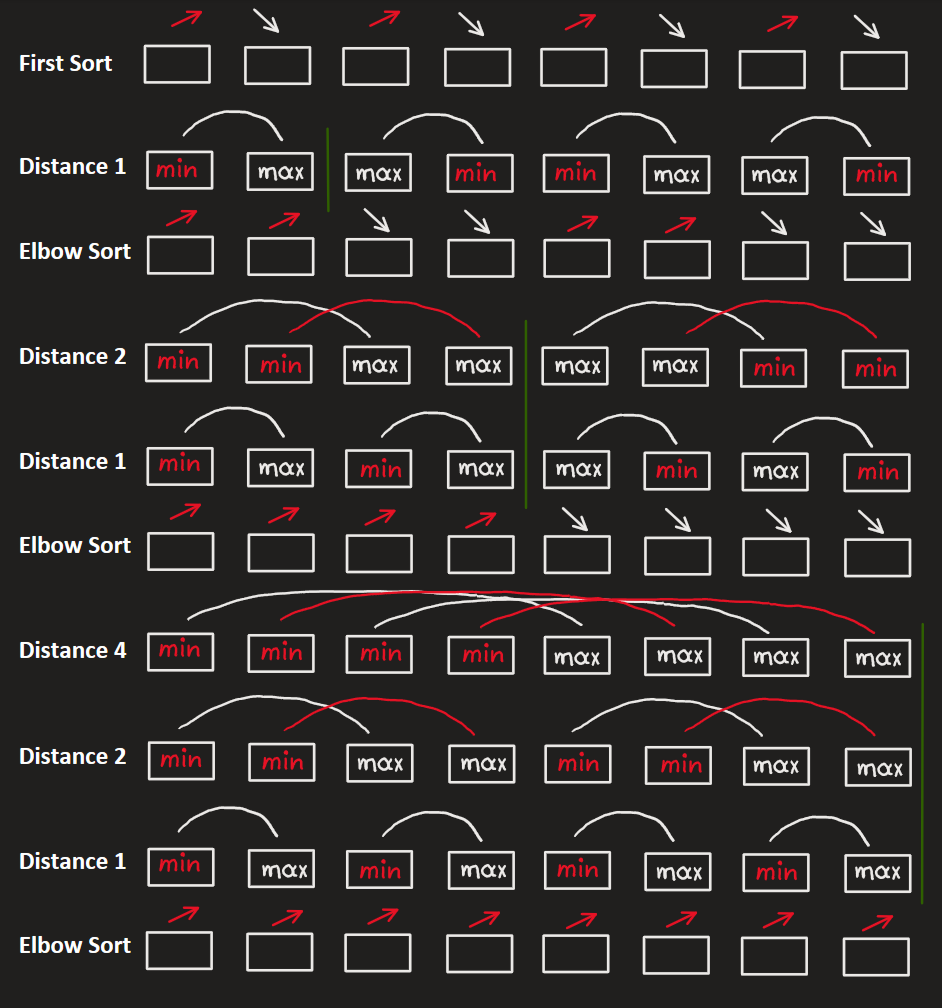
\includegraphics[width=0.9\linewidth]{distributedBitonic.png}
    \caption{Example of Distributed Bitonic Sort for 8 processes}
    \label{fig:enter-label}
\end{figure}

In the above figure, each rectangle represents a process. Each row is a step of the algorithm, and it is either a communication step or a sorting step.

\subsection{Partner}
The rank of the \texttt{partner} process can be easily calculated using the current communication \texttt{distance} and the local process's rank. The \texttt{distance} depends on the current \texttt{stage} of the algorithm and is always a power of two, ranging between \( 2^{\text{stage}-1} \text{ and } 2^0 \). Below is a reference table of the \texttt{partner} pairs as they are formed by the following experession:

\[\text{rank} \oplus \text{distance}\]
\begin{table}[h]
    \centering
    \begin{tabular}{|c|c|c|c|c|}
        \hline
        \textbf{Decimal} & \textbf{Binary} & \textbf{XOR with distance 1} & \textbf{XOR with distance 2} & \textbf{XOR with distance 4} \\ \hline
        0 & 000 & 001 & 010 & 100 \\ \hline
        1 & 001 & 000 & 011 & 101 \\ \hline
        2 & 010 & 011 & 000 & 110 \\ \hline
        3 & 011 & 010 & 001 & 111 \\ \hline
        4 & 100 & 101 & 110 & 000 \\ \hline
        5 & 101 & 100 & 111 & 001 \\ \hline
        6 & 110 & 111 & 100 & 010 \\ \hline
        7 & 111 & 110 & 101 & 011 \\ \hline
    \end{tabular}
    \caption{XOR Table}
    \label{tab:xor}
\end{table}

\subsection{Exchange Data}
Communication between processes is achieved through the \texttt{exchange} function. Each process uses \texttt{MPI\_Sendrecv} to send its local data to its partner and store the received data from the partner in a buffer called \texttt{remote}.
\vspace{0.3cm}
\begin{lstlisting}[language=C]
    Sequence exchange(int partner, Sequence local)
    {
        Sequence remote = createSeq(local.size);
        MPI_Sendrecv(local.arr, local.size, MPI_INT, partner, 0, remote.arr, remote.size, MPI_INT, partner, 0, MPI_COMM_WORLD, MPI_STATUS_IGNORE);
        return remote;
    }
\end{lstlisting}
\newpage
\subsection{Maxima or Minima}
After receiving data from its remote partner, each process performs an element-wise comparison between its local elements and the remote ones. It then keeps either the \textbf{minimums} or the \textbf{maximums}. This decision is crucial for the final result and depends on the current \texttt{stage} and \texttt{distance}.

The algorithm behind this decision-making can be better understood through a mirror analogy. At each \texttt{stage}, a mirror is placed in front of the process with rank \( 2^{\text{stage}} \). These mirrors, represented by green vertical lines in \textbf{Figure 2}, have a width of \( 2 \times 2^{\text{stage}} \). The processes with ranks in the range \([0, 2^{\text{stage}} - 1]\) are \textbf{reflections} of those with ranks in the range \([2^{\text{stage}}, 2 \times 2^{\text{stage}} - 1]\). This pattern repeats until the end of the global sequence.

To identify a process’s reflection within this mirror system, we first calculate its position relative to the mirror’s width using: \texttt{pos} = \texttt{rank \% w} ,where \( w = 2 \times 2^{\text{stage}} \).

Using this position, the reflection is computed as:
\begin{itemize}
    \item For processes on the left of the mirror (\( \texttt{pos} < \texttt{mirror} \)), the reflection is \( \texttt{mirror} - \texttt{pos} - 1 \).
    \item For processes on the right (\( \texttt{pos} \geq \texttt{mirror} \)), the reflection is \( \texttt{pos} - \texttt{mirror} \).
\end{itemize}

With the reflection determined, the decision to keep either the \textbf{minimums} or the \textbf{maximums} is based on the \texttt{distance}. Specifically, the algorithm examines the \( \log_2(\texttt{distance}) \)-th bit (counting from the right) of the process's rank:
\begin{itemize}
    \item If the bit is \( 0 \), the process retains the \textbf{maximums}.
    \item If the bit is \( 1 \), it retains the \textbf{minimums}.
\end{itemize}

\vspace{0.3cm}
\begin{lstlisting}[language=C]
void minmax(int rank, int stage, int distance, Sequence local, Sequence remote)
{
    int mirror = 1 << stage;
    int w = 2 * mirror;
    int pos = rank % w;

    int reflection = pos < mirror ? mirror - pos - 1 : pos - mirror;

    if (reflection & (1 << (int)log2(distance))){
        // Keep min elements (element-wise)
    }
    else{
        // Keep max elements (element-wise)
    }
}

\end{lstlisting}
\newpage
Below is a reference table that illustrates the logic for \texttt{stage} 2 of the \texttt{Distributed Bitonic Sort} with 8 processes. In this \texttt{stage}, there are two communication \texttt{step}s. The first \texttt{step} involves a \texttt{distance} of 2, and the second \texttt{step} involves a \texttt{distance} of 1. In both \texttt{step}s, a single mirror is ``placed'' in front of rank 4.

During the first communication \texttt{step}, the decision to retain either the minimums or maximums is based on the second bit from the right of the process's rank. In the second communication \texttt{step}, this decision is made using the first bit from the right of the rank.

\begin{table}[h]
    \centering
    \begin{tabular}{|c|c|c|c|c|}
        \hline
        \textbf{Decimal} & \textbf{Rank} & \textbf{Reflection} & \textbf{Distance 1} & \textbf{Distance 2} \\ \hline
        0 & 000 & 0\textcolor{blue}{1}\textcolor{blue}{1} & \textcolor{blue}{min} & \textcolor{blue}{min} \\ \hline
        1 & 001 & 0\textcolor{blue}{1}\textcolor{red}{0} & \textcolor{red}{max} & \textcolor{blue}{min} \\ \hline
        2 & 010 & 0\textcolor{red}{0}\textcolor{blue}{1} & \textcolor{blue}{min} & \textcolor{red}{max} \\ \hline
        3 & 011 & 0\textcolor{red}{0}\textcolor{red}{0} & \textcolor{red}{max} & \textcolor{red}{max} \\ \hline
        4 & 100 & 0\textcolor{red}{0}\textcolor{red}{0} & \textcolor{red}{max} & \textcolor{red}{max} \\ \hline
        5 & 101 & 0\textcolor{red}{0}\textcolor{blue}{1} & \textcolor{blue}{min} & \textcolor{red}{max} \\ \hline
        6 & 110 & 0\textcolor{blue}{1}\textcolor{red}{0} & \textcolor{red}{max} & \textcolor{blue}{min} \\ \hline
        7 & 111 & 0\textcolor{blue}{1}\textcolor{blue}{1} & \textcolor{blue}{min} & \textcolor{blue}{min} \\ \hline
    \end{tabular}
    \caption{Stage 2 for 8 processes}
    \label{tab:xor}
\end{table}

\subsection{Ascending or Descending}
At the end of every \texttt{stage}, each process sorts its elements in ascending or descending order. The function \texttt{ascdesc} defines this order in a manner similar to the approach used previously with the reflection. For example, in the first sort (stage 0), we keep the first bit from the right. If this bit is equal to zero, the process sorts its local array in ascending order; otherwise, it sorts it in descending order.
\[\texttt{rank} \ \&  \ (1 \ll \texttt{stage})\]

\subsection{Elbow Sort}
At the end of each stage, all processes hold a bitonic sequence. To increase time efficiency, the \texttt{Distributed Bitonic Sort} algorithm takes advantage of this characteristic and uses \texttt{elbowSort} for sorting instead of \texttt{qsort}.

The \texttt{elbowSort} function takes a bitonic sequence as an input and sorts it in the desired order, designated by the \texttt{ascdesc} function. It begins by identifying the \textbf{"elbow"} of the bitonic sequence, which is defined as the element for which all elements before it are monotonically decreasing (or increasing), and all elements after it are monotonically increasing (or decreasing). 

It is important to note that only the \textbf{minimum} or \textbf{maximum} elements can serve as the elbow of the sequence. If these elements were placed elsewhere, they would disrupt the monotonic increase or decrease, which is a required property for the sequence to be considered bitonic. Furthermore, sequences like \([6, 4, 3, 1, 2, 5, 8, 7]\) are still considered bitonic sequences because they always have a cyclic rotation with a correct elbow candidate, such as this one \([7, 6, 4, 3, 1, 2, 5, 8]\).

For this implementation, we have chosen to consider the \textbf{minimum} element as the elbow and take advantage of the fact that all the elements before and after it are already sorted. We start by placing the elbow in the correct position which according to the sorting order, is either at the start of the sequence, if sorting in ascending order, or at the end of it, if sorting in descending order. After that, we place \textbf{two pointers}: one to the \textbf{left} and one to the \textbf{right} of the elbow.
\vspace{0.3cm}
\begin{lstlisting}[language=C]
    int l = (elbowIndex - 1 + s.size) % s.size;
    int r = (elbowIndex + 1) % s.size;
\end{lstlisting}
\vspace{0.3cm}
The algorithm then compares the elements at the two pointers. The smaller element of the two will take the next position in the sequence and its corresponding pointer will then move one step to the right (if referring to the right pointer) or one step to the left (if referring to the left pointer). This process continues until the entire sequence is sorted.

When a pointer reaches the end of the sequence, it wraps around to the beginning (and vice versa for the opposite pointer) to ensure that cases like the one we mentioned earlier are sorted correctly.

\vspace{0.3cm}
    \begin{lstlisting}[language=C]
    // Sorting in ascending order
    int sortedIndex = 0;
    sortedSeq.arr[sortedIndex++] = s.arr[elbowIndex];
    
    while (sortedIndex < s.size)
    {
        if (s.arr[l] < s.arr[r])
        {
            sortedSeq.arr[sortedIndex++] = s.arr[l];
            // Wrap around to end if l < 0
            l = (l - 1 + s.size) % s.size;
        }
        else
        {
            sortedSeq.arr[sortedIndex++] = s.arr[r];
            // Wrap around to start if r >= s.size
            r = (r + 1) % s.size;
        }
    }
\end{lstlisting}
\newpage
\section{Results}
For testing, we executed our program on the \textbf{Rome} partition of the \textbf{Aristotle cluster}, provided by Aristotle University of Thessaloniki. The Rome partition consists of 17 nodes with 128 CPU cores per node. To test our implementation at high scale ranged, we utilized all 128 CPU cores of a single node, and the following results were obtained:

\begin{figure}[H]
    \centering
    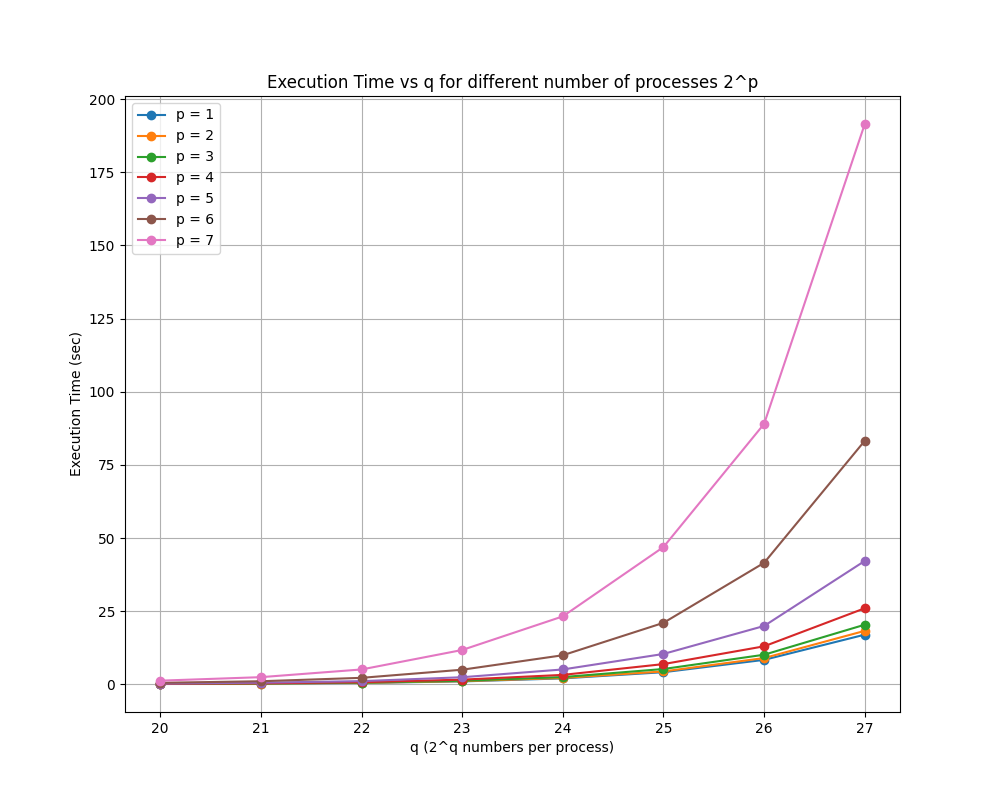
\includegraphics[width=0.9\linewidth]{results.png}
    \caption{Performance of Distributed Bitonic Sort}
    \label{fig:enter-label}
\end{figure}

To verify the speedup of our algorithm, we have created the following plot comparing the performance of \texttt{qsort} and the serial implementation of \texttt{Bitonic Sort} against \texttt{Distributed Bitonic Sort} across different datasets (varying values of \(q\)). The plot clearly demonstrates that \texttt{Distributed Bitonic Sort} outperforms both \texttt{qsort} and serial \texttt{Bitonic Sort}. While the speedup for \(p=1\) is minimal, the speedup becomes significant as the number of processes increases, particularly for datasets where \(q=21\) and \(q=22\).

\begin{figure}[H]
    \centering
    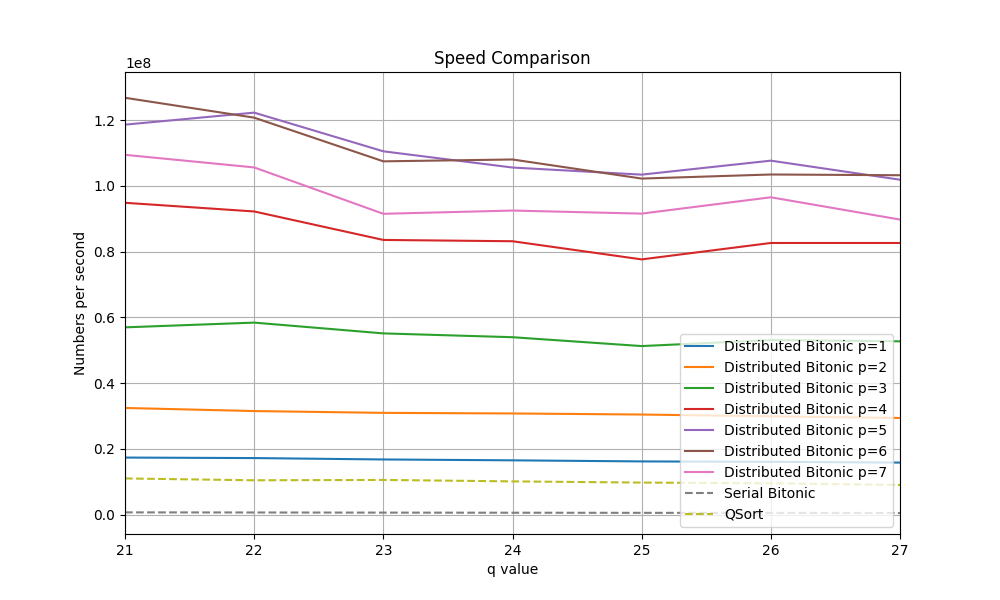
\includegraphics[width=0.9\linewidth]{speed.png}
    \caption{Speed comparison against \texttt{qsort} and serial Bitonic Sort}
    \label{fig:enter-label}
\end{figure}

\section{Conclusion}

In this report, we explored the implementation of the \texttt{Distributed Bitonic Sort} algorithm, with a focus on leveraging parallelism through \texttt{MPI} to optimize sorting tasks in a distributed environment. The results demonstrated the scalability of our approach, showcasing the potential of \texttt{MPI} to significantly accelerate algorithms as the number of processes increases.

\end{document}
